\section{Experimental Results}\label{sec:crosscorr_experiments}

To evaluate the performance of the proposed algorithms and optimizations, we performed extensive benchmarks covering the vast configuration space of optimization combinations, input sizes, and individual attuning parameters. In this section, we summarize the performance results of the described optimizations and compare them with each other to find the optimal one for each input size and problem configuration. In the end, we also compare our methods with the asymptotically better FFT-based algorithm to find the limits of definition-based algorithms.

% -----------------------------------------------------------------------------
\subsection{Experimental setup}
% -----------------------------------------------------------------------------

We carried out the experiments on three different NVIDIA GPUs representing three different architectures: Tesla V100 SXM2 32 GB (Volta arch.), Tesla A100 PCIe 80 GB (Ampere arch.), and Tesla L40 PCIe 48 GB (Ada Lovelace arch.). The systems were using CUDA 12.2 with driver version 535.104.05. Each single benchmark was repeated $10$ times, each time running for at least $0.1$ seconds. This setup was necessary to ensure proper measurement of short-running kernels. After removing the outliers, and checking that the remaining measurements have reasonable variance, the arithmetic mean of the remaining values was taken as the final result to be presented.

The results of all three GPUs do not differ significantly. The figures further presented in the paper cover only the results of the Tesla A100 GPU. The complete result set is available in our replication package\footnote{\url{https://github.com/asmelko/jpdc23-artifact}}.

\subsubsection{FFT-based algorithm}

In the following discussion, we also compare our proposed algorithms with the FFT-based approach. As described in Section~\ref{sec:cross_corr_fft}, the FFT-based algorithm runs in 5 steps: Input padding, Discrete Fourier Transform (DFT), Hadamard product, Inverse DFT and quadrant swap. We used highly optimized cuFFT routines for DFT and Inverse DFT. The Hadamard product was implemented in a custom kernel since it is an embarrassingly parallelizable algorithm. We chose to omit the quadrant swap from the measurements since this step is not generally required for all cross-correlation use cases (e.g. when the correlation result is processed further and the swap can be amortized in a subsequent step).

The DFT routines operate on a \emph{cuFFT plan} --- an opaque data structure, which needs to be initialized beforehand. Although we can only speculate what operations the plan initialization exactly performs, cuFFT documentation states that it also allocates GPU memory. The allocation is quite time-consuming in comparison to the kernel execution, so we decided to plot it separately to provide a more accurate picture of the relative performance. We plotted the FFT-based algorithm performance in two variants --- \emph{fft} aggregates the runtime of DFT, Hadamard product, and Inverse DFT; the \emph{fft+plan} also includes the time required for the plan creation. The \emph{fft+plan} presents a time that would be closer to a realistic application. The \emph{fft} shows the theoretical limits of the FFT-based approach that may be relevant if the initialization phase can be amortized or the cuFFT plan data structure can be re-used for many computations.
% Note, that comparing kernel runtimes to memory allocations is not generally fair, but in our case the allocation is an extra step in the FFT algorithm and therfore it is worthy the overall comparison.

% -----------------------------------------------------------------------------
\subsection{One-to-one benchmarks}
% -----------------------------------------------------------------------------

The one-to-one configuration can be solved using either the \emph{warp-shuffle} algorithm (possibly with the \emph{grouped-overlap} or \emph{split-row} optimization) or the \emph{warp-per-overlap} algorithm. First, we evaluate \emph{grouped-overlap} and \emph{split-row} optimizations separately to determine optimal tuning parameters. Afterward, we present the overall comparison of all methods including the na\"{i}ve \emph{overlap-wise} algorithm (baseline) and the FFT-based algorithm.

\subsubsection{Grouped-overlap}
%\paragraph{\textbf{\emph{grouped-overlap}}}

In this micro-benchmark, we present normalized times per single FMA operation (with amortized data transfers). To ensure reasonably interpretable values, we needed to saturate the GPU cores completely (i.e., generate enough workload even if the inputs are small). This prevents a misleading observation when an increase in the grouping factor (which improves efficiency) could be perceived as a decrease in the apparent FMA throughput just because the GPU gets undersaturated. We manually modified the kernel of the algorithm to run $4000$ copies of the input problem in a single grid. This allows us to correctly measure the actual FMA throughput, but the results are not directly comparable with other methods, especially in the case of very small inputs.

The results are shown in Figure~\ref{fig:grouped-overlap}. By increasing the number of grouped overlaps (and hence increasing the caching and data reuse factor), the optimization performs better for all matrix sizes. We can also observe that the algorithm performs significantly better for larger inputs, which is caused by the inherent limitation of the warp-shuffle principle. Very small matrices (like $16\times 16$) struggle with GPU underutilization and code divergence as the threads in a warp become idle for a considerable amount of time. With the larger inputs, the thread utilization becomes better and once exceeding $64\times 64$, the warp-shuffle algorithm can fully utilize the warp-wise buffer for the left matrix (as described in Section~\ref{sec:ws-algo}).

%We can also observe the diminishing effects of increasing the parameter values --- for $16\times 16$ matrix, a drastic data reuse of $8\times 8$ variant significantly reduces the number of jobs required to compute the output matrix. Since our implementation assigns output matrix computation to CUDA blocks, the number of participating threads in a block is bellow the optimal number of threads that are able to run in parallel on a single streaming multiprocessor.

% For bigger matrices, $8\times 8$ parameter variant starts to show the similar apparent speedup that the other variants. For matrices in the middle of the measured range, the speedup builds slower for $8\times 8$ than for the other variants because of the unfavorable initial+final phase to main phase ratio of \emph{grouped-overlap} algorithm.

% The figure also shows a rather big increase in FMA throughput for bigger matrices compared to the small ones. Very probably, this is caused by the warp-wise buffers. For small matrices, some registers in the $64$ registers-wide buffer will be unused while requiring the same number of costly global memory accesses. The buffer will reach the full utilization for $64\times 64$ matrices, which explains the steep slope ending at that data point. We still see the FMA throughtput increase and stabilize near $128\times 128$ sizes, caused by the stabilization of the internal ratio of global loads to buffer rotations mentioned in Section TODO.

For the sake of brevity, we do not show the plot measuring the influence of the block size on the performance of the algorithm (it is available in our replication package). The results conclusively show that as soon as the block size reaches a sufficient level to fully utilize a GPU streaming multiprocessor, the performance of the algorithm is not affected by increasing it further. Therefore, we used the block size of $4$ warps ($4\times 32$) for all the experiments.

\begin{figure}[ht]
	\begin{minipage}{.48\textwidth}
		\centering
		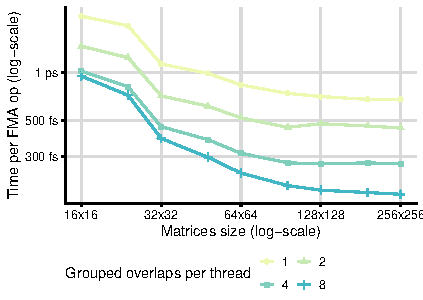
\includegraphics[width=\textwidth]{crosscorr/plots/one-to-one/grouped-overlap.pdf}
		\caption{The \emph{grouped-overlap} results, normalized times (per FMA) for completely saturated GPU}
		\label{fig:grouped-overlap}
	\end{minipage}%
	\begin{minipage}{.03\textwidth}~
	\end{minipage}
	\begin{minipage}{.48\textwidth}
		\centering
		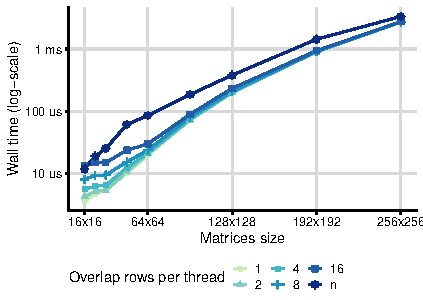
\includegraphics[width=\textwidth]{crosscorr/plots/one-to-one/split-row.pdf}
		\caption{The \emph{split-row} benchmark on various inputs, absolute (wall) times}
		\label{fig:split-row}
	\end{minipage}
\end{figure}

\subsubsection{Fine-grained parallelism}
% \paragraph{\textbf{\emph{split-row}}}

When problem size is not sufficient to saturate the GPU, a fine-grained parallelism is required. One possibility is to employ the \emph{split-row} optimization for the warp-shuffle algorithm, which splits each Hadamard product into multiple independently processed stripes. Figure \ref{fig:split-row} shows the performance for different job granularity levels ranging from the finest job of $1$ row per thread to $n$ (all) per thread (no splitting takes place --- i.e., referring to basic warp-shuffle implementation). As expected, the finest granularity helps the most for the smallest matrices and the speedup over $n$ (baseline) variant progressively diminishes as the input size increases (and thus saturates the GPU without splitting).

%\paragraph{\textbf{\emph{warp-per-overlap}}}
The alternate approach (\emph{warp-per-overlap} algorithm) has no tuning parameters, so we do not provide a separate micro-benchmark for it. The comparison of both algorithms is evaluated in the following.

\subsubsection{Comparison of all one-to-one solutions}
%\paragraph{\textbf{One-to-one optimizations comparison}}

Figure~\ref{fig:one-to-one} (left) summarizes the performance of the discussed one-to-one algorithms. The \emph{baseline} algorithm denotes the na\"{i}ve \emph{overlap-wise} implementation (one thread per one overlap with no data reuse) which we use as a baseline. Algorithms, which have tuning parameters, use their optimal values for given input sizes (as determined in the previous micro-benchmarks).

\begin{figure}[ht]
	\centering
	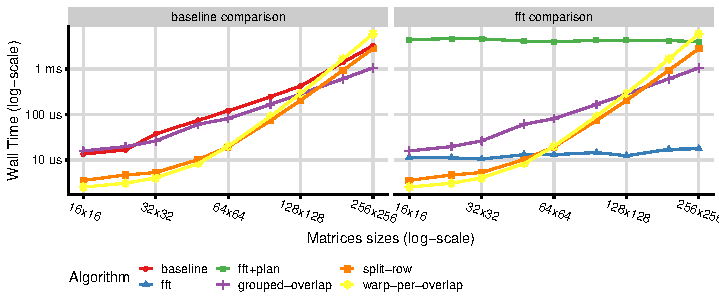
\includegraphics{crosscorr/plots/one-to-one/one-to-one.pdf}
	\caption{Comparison of one-to-one algorithms}
	\label{fig:one-to-one}
\end{figure}

The \emph{grouped-overlap} optimization is the most beneficial for larger matrices while for smaller matrices it suffers the low GPU occupancy due to the insufficient amount of tasks. The \emph{split-row} and \emph{warp-per-overlap} algorithms perform better on smaller matrices as they resolve the occupancy issue. The \emph{warp-per-overlap} performs better on very small inputs as it was designed specifically to prefer core occupancy over data caching. The \emph{split-row} optimization of the \emph{warp-shuffle} algorithm performs slightly worse for matrices smaller than $64\times64$; for larger matrices, the data reuse and coalesced loads become more important, so it outperforms \emph{warp-per-overlap}. Overall, the proposed optimizations perform better than baseline \emph{overlap-wise} algorithm, being $5.3\times$ faster for $16\times16$ input and $3.1\times$ faster for $256\times 256$ input.

% \paragraph{\textbf{Comparison with FFT}}

%Finally, we compare the proposed optimizations against the FFT-based algorithm, in our case the highly optimized CUDA library \emph{cuFFT}~\cite{site:cufft}. Recalling from Section~\ref{sec:cross_corr_fft}, FFT based algorithm must perform the input padding, Discrete Fourier Transform (DFT), Hadamard product, Inverse DFT and quadrant swap. We used cuFFT optimized routines for DFT and Inverse DFT. For Hadamard product, we implemented the custom kernel (Hadamard product is an embarrassingly parallelizable algorithm and its implementation details were omitted for brevity).

%In order to provide less convoluted and fairer results, we decided not to include padding and quadrant swap into the benchmark. We chose to omit the quadrant swap because this step is not generally required for every cross-correlation usecases; e.g., in digital image cross-correlation, only the maximum of the cross-correlation matrix is needed. Skipping quadrant swap therefore makes it more fair comparison with definition-based algorithms. Regarding the paddings, it is a simple operation that may influence the performance very little, so we omitted it for the simplicity of the benchmarking code.

%The DFT routines operate on a \emph{cuFFT plan} --- an opaque data structure, which needs to initialized beforehand. Although we can only speculate what operations does plan initialization exactly performs, cuFFT documentation states that it allocates GPU memory. The allocation takes multiple magnitudes longer than the kernel runtimes, so we decided to plot it separately to provide the better picture of the speedups. We plotted FFT-based algorithms in two variants --- \emph{fft}, which shows the aggregated runtime of DFT, Hadamard product and Inverse DFT, and \emph{fft+plan}, which also adds the plan creation to the sum. Note, that comparing kernel runtimes to memory allocations is not generally fair, but in our case the allocation is an extra step in the FFT algorithm and therfore it is worthy the overall comparison.

The right part of Figure~\ref{fig:one-to-one} reveals that the cuFFT plan creation is the most costly part of the algorithm, dominating the runtime in each measured data point. When the initialization is taken into account, the definition-based approach appears much better in the terms of performance. The turning point, where the \emph{fft+plan} surpasses our optimizations, seems to be around $384\times 384$ matrix. When considering \emph{fft} alone, only the \emph{warp-per-overlap} algorithm outperforms it (having $4.5\times$ speedup on $16\times 16$ inputs) and the turning point is around $48\times 48$.


% -----------------------------------------------------------------------------
\subsection{One-to-many benchmarks}
% -----------------------------------------------------------------------------

The \emph{one-to-many} and \emph{n-to-mn} scenarios enable utilization of the \emph{multi-matrix-right} optimization of the warp shuffle algorithm. This optimization can be combined with \emph{grouped-overlap} or \emph{split-row}, so we present their respective performance evaluation in detail.

We did not include the \emph{warp-per-overlap} evaluation in this section, because it does not provide any additional improvement in terms of performance. The additional workload of multiple cross-correlations mitigates the need for extremely fine-grained parallelism, so the \emph{split-row} optimization is more than sufficient even for the smallest matrices.

\subsubsection{Multi-matrix-right with grouped-overlap}
% \paragraph{\textbf{\emph{multi-matrix-right grouped-overlap}}}

In this configuration, we are benchmarking the one-to-many scenario with $4000$ right matrices, which completely saturates the GPU. The left subplot of Figure~\ref{fig:multimat-right-grouped-overlap} shows the \emph{grouped-overlap} results without the \emph{multi-matrix-right} optimization. In the middle and the right subplot, the number of right matrices per thread is $2$ and $4$ respectively (i.e., enabling the multi-matrix caching). The results indicate that increasing the number of right matrices per thread does not collide with the data reuse made by the \emph{grouped-overlap} optimization and both optimizations can work in synergy.

\begin{figure}[ht]
	\centering
	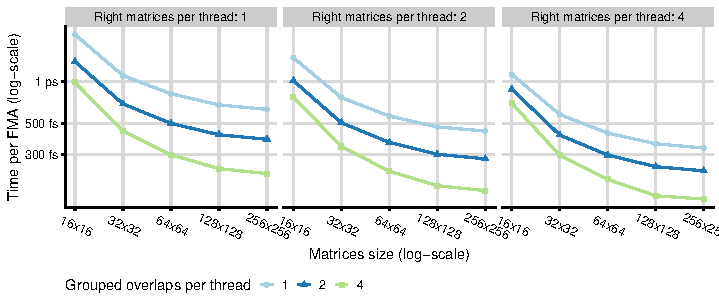
\includegraphics{crosscorr/plots/one-to-many/multimat-right-grouped-overlap.pdf}
	\caption{\emph{Multi-matrix-right}+\emph{grouped-overlap} results (one-to-many, $4000$ right matrices)}
	\label{fig:multimat-right-grouped-overlap}
\end{figure}

Considering a sufficient total number of the right matrices, we can increase the factor of right matrices per thread significantly more and still expect the performance to improve. The primary limitation is the maximum number of registers per thread a GPU allows to allocate. The required number of registers increases linearly with the product of right matrices per thread used by \emph{multi-matrix-right} and warp-wise buffers used by the \emph{grouped-overlap} (which is about $3 \cdot 4^2$ registers per thread for the variant that reuses the data the most intensively in Figure~\ref{fig:multimat-right-grouped-overlap}). When the maximum is exceeded, the GPU resorts to register spilling (offloading to local memory), which harms the performance significantly.

We have observed that the parameter values presented in Figure~\ref{fig:multimat-right-grouped-overlap} are in a reasonable range. Increasing the grouping factor or number of right matrices further does not help much with performance on current GPU architectures, but it creates additional issues with the compilation (especially bloating the size of our artifact). Hence, we have excluded higher values from the presented results for practical reasons.


\subsubsection{Multi-matrix-right with split-row}
% \paragraph{\textbf{\emph{multi-matrix-right split-row}}}

This micro-benchmark was designed to determine how the combination of multi-matrix data reuse and fine-grained parallelism can improve performance. In theory, applying \emph{multi-matrix-right} on small inputs may decrease the performance because it groups tasks, thus limiting the parallelism. Combining multi-matrix optimization with \emph{split-row} may provide enough parallel GPU work whilst improving the data reuse.

\begin{figure}[ht]
	\centering
	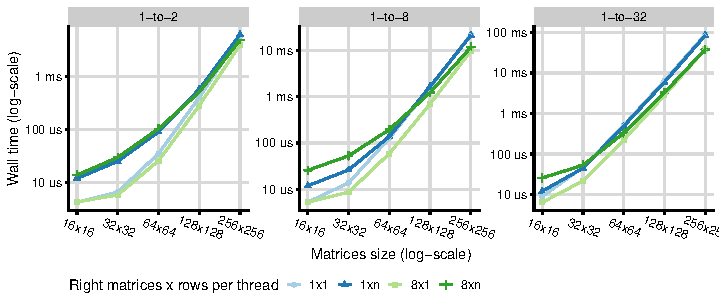
\includegraphics{crosscorr/plots/one-to-many/multimat-right-split-row.pdf}
	\caption{\emph{Multi-matrix-right}+\emph{split-row} benchmark results (please note that the $8\times1$ and $8\times n$ parametrizations are in fact $2\times1$ and $2\times n$ in the \emph{1-to-2} scenario since we can cache only up to the total number of right matrices)}
	\label{fig:multimat-right-split-row}
\end{figure}

%We ploted the optimization combination in Figure~\ref{fig:multimat-right-split-row}. If we compare only \emph{multi-matrix-right} optimization without \emph{split-row} (a triangle and a cross in each subplot), we can see that a big data reuse (cross) decreases the performance for small matrix sizes. But if we look at their \emph{split-row} alternatives (a circle and a square in each subplot), we can see that finer sized jobs counter the performance degradation caused by the data reuse. Ultimately, when the problem size is bigger and a GPU is saturated, these alternatives meet (circles meet with triangles and squares meet with crosses) and the performance is the same.
Figure~\ref{fig:multimat-right-split-row} demonstrates how the \emph{split-row} improves performance for small problem sizes. The $1\times n$ and $8\times n$ denote the versions that do not take advantage of \emph{split-row} (the size of row-stripes is $n$, which stands for the size of the overlapping area). The $1\times 1$ and $8\times 1$ stand for the most fine-grained versions of \emph{split-row} (one task takes only one row). The data indicate that in the extreme, the speedup caused by splitting the rows could reach an order of magnitude ($16\times16$ with a low number of right matrices). Furthermore, the $8\times 1$ parametrization (i.e., the most fine-grained division that caches $8$ right matrices) exhibits the best performance over the examined domain.

\subsubsection{Comparison of one-to-many optimizations}
%\paragraph{\textbf{One-to-many optimizations comparison}}

The overall comparison is presented in Figure~\ref{fig:one-to-many}. Similarly as for one-to-one optimizations, the \emph{split-row} dominates the small matrices and \emph{grouped-overlap} dominates the larger matrices. Employing \emph{multi-matrix-right} (especially when combined with \emph{split-row}) shifts the turning point where higher data reuse wins over more granular jobs. Using $32$ right matrices, we achieve $11.8\times$ speedup over na\"{i}ve \emph{overlap-wise} (baseline) algorithm for $16\times 16$ input and $6\times$ speedup for $256\times 256$ input.

When we compare the best definition-based algorithm with cuFFT, the \emph{split-row} still outperforms \emph{fft} for extra small matrices. The turning point for \emph{fft+plan} is slightly beyond the size of $256\times 256$ for $2$ input matrices, and $128\times 128$ for $32$ input matrices.

\begin{figure}[ht]
	\centering
	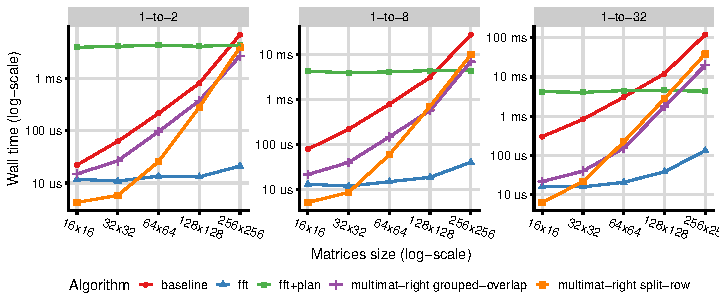
\includegraphics{crosscorr/plots/one-to-many/one-to-many.pdf}
	\caption{Comparison of one-to-many algorithms}
	\label{fig:one-to-many}
\end{figure}


\subsubsection{Extending one-to-many into n-to-mn}

The \emph{n-to-mn} problem is in fact $n$ instances of \emph{one-to-many} problem. There are two ways of extending the \emph{one-to-many} implementation --- we could either simply run the original kernel $n$ times simultaneously or create a new kernel that takes an additional index. After a careful analysis, we found no additional benefits of implementing a separate kernel. When running \emph{one-to-many} kernel $n$ times, the only issue worth mentioning is that the runtime must utilize a sufficient amount of CUDA streams, so the execution of the kernels may overlap in case the individual invocations cannot saturate the GPU.

The overhead of the simultaneous kernel execution is negligible, so we have omitted figures with the performance results from the paper for the sake of brevity. The data and the plots may be found in the attached replication package.


% -----------------------------------------------------------------------------
\subsection{n-to-m benchmarks}
% -----------------------------------------------------------------------------

This scenario allows the most elaborate data reuse pattern called the \emph{multi-matrix-both} optimization. Similarly to \emph{multi-matrix-right}, it can be combined with \emph{grouped-overlap} or \emph{split-row}.

\subsubsection{Multi-matrix-both with grouped-overlap}
%\paragraph{\textbf{\emph{multi-matrix-both grouped-overlap}}}

In Figure~\ref{fig:multimat-both-grouped-overlap}, we present the results of \emph{grouped-overlap} alone (left subfigure), combined with \emph{multi-matrix-right} (center subfigure), and with \emph{multi-matrix-both} (right subfigure). Regardless of the number of grouped overlaps, the \emph{multi-matrix} optimization alone improves the speedup, and the combination of both optimizations exhibits the best performance. In the case of the highest overlap grouping, the speedup of \emph{both} variant over \emph{right} variant is about $1.75\times$ on all input sizes.

\begin{figure}[ht]
	\centering
	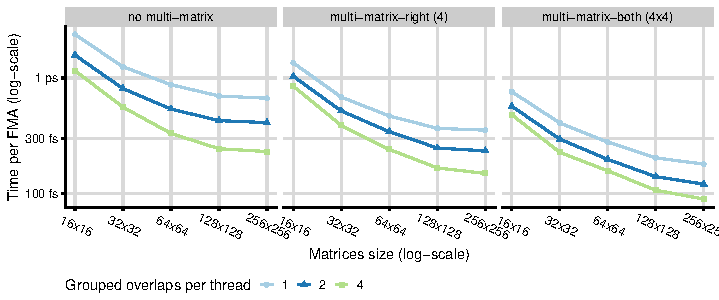
\includegraphics{crosscorr/plots/n-to-m/multimat-both-grouped-overlap.pdf}
	\caption{\emph{Multi-matrix-both}+\emph{grouped-overlap} benchmark results ($128$-to-$128$ matrices)}
	\label{fig:multimat-both-grouped-overlap}
\end{figure}


\subsubsection{Multi-matrix-both with split-row}
%\paragraph{\textbf{\emph{multi-matrix-both split-row}}}

Similarly to \emph{multi-matrix-right} combination, we aim at verifying that \emph{split-row} optimization enables the data reuse on smaller matrices without any performance downgrade. We tested this on two different matrix counts: $2$-to-$2$ and $8$-to-$8$ matrices (top and bottom pair of subfigures in Figure~\ref{fig:multimat-both-split-row} respectively). The results indeed show that for small matrices, the \emph{multi-matrix} alone (the left pair of subfigures) is slower than the \emph{multi-matrix} combined with \emph{split-row} (the right pair of subfigures). The speedup of finer parallelism for $16\times16$ matrix and the highest --- about $5\times$. As expected, the speedup gets negligible for larger matrices.

\begin{figure}[ht]
	\centering
	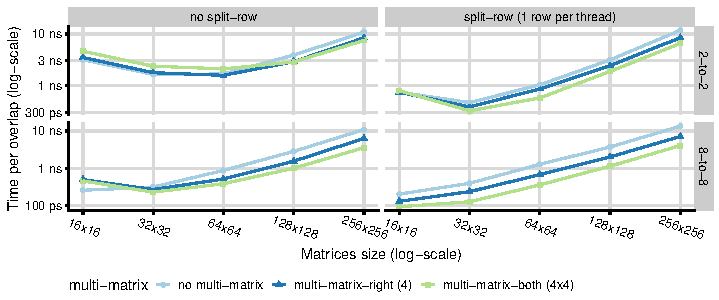
\includegraphics{crosscorr/plots/n-to-m/multimat-both-split-row.pdf}
	\caption{\emph{Multi-matrix-both}+\emph{split-row} benchmark results}
	\label{fig:multimat-both-split-row}
\end{figure}

\subsubsection{Comparison of n-to-m optimizations}
%\paragraph{\textbf{n-to-m optimizations comparison}}

The overall comparison is presented in Figure~\ref{fig:n-to-m}. Similarly to \emph{one-to-many} optimizations, the \emph{split-row} dominates smaller inputs while \emph{grouped-overlap} dominates larger inputs. However, when the multi-matrix factor gets higher ($32$-to-$32$ matrices), the \emph{grouped-overlap} gets more efficient than \emph{split-row} as the GPU is already saturated and data reuse becomes more important.

Another observation is that cuFFT gets better even for slightly smaller matrices when the number of cross-correlations is growing. That is a natural conclusion of the fact that the cuFFT plan initialization takes constant time, so it gets more amortized into the overall computation. For $32$-to-$32$ matrices, the turning point gets as low as $64\times 64$ matrices.

\begin{figure}[ht]
	\centering
	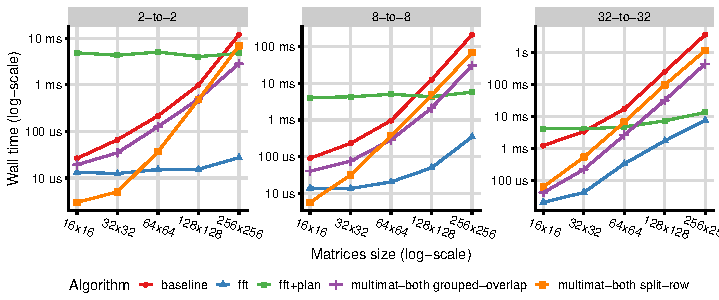
\includegraphics{crosscorr/plots/n-to-m/n-to-m.pdf}
	\caption{Comparison of n-to-m algorithms on various inputs.}
	\label{fig:n-to-m}
\end{figure}


% -----------------------------------------------------------------------------
\subsection{Summary and outcomes}
% -----------------------------------------------------------------------------

To summarize the empirical results, we provide basic guidelines for selecting the optimal algorithm and its optimization. Table~\ref{tab:overview-all} presents the algorithm of choice for given scenarios (rows) and matrix sizes (columns). The \emph{one-to-many} instances implicitly assume utilization of \emph{multi-matrix-right} optimization and the \emph{n-to-m} always employ \emph{multi-matrix-both} optimization.

As indicated in the previous benchmarks, the smallest configurations benefit from \emph{split-row} optimization (or the \emph{warp-per-overlap} algorithm, in case of \emph{one-to-one} scenario). The middle-sized problems can benefit from the \emph{grouped-overlap} optimization and the largest problems should switch to the FFT-based approach which is asymptotically better.

Please note that the turning points for each configuration are not exact and they may differ slightly across the GPU architectures.

\begin{table}
	\begin{tabular}{l|cccccccc}\toprule
		             & $16^2$                                     & $32^2$                                & $64^2$                                & $128^2$         & $192^2$                     & $256^2$ & $384^2$ & $\infty$ \\\midrule
		\emph{1-to-1}   & \multicolumn{3}{c|}{\texttt{warp-overlap}} & \multicolumn{1}{c|}{\texttt{split}}   & \multicolumn{3}{c|}{\texttt{grouped}} & \multicolumn{1}{r}{\texttt{fft+p}}                                \\\bottomrule
		\emph{1-to-2}   & \multicolumn{4}{c|}{\texttt{split}}        & \multicolumn{2}{c|}{\texttt{grouped}} & \multicolumn{2}{c}{\texttt{fft+p}}                                                                        \\
		\emph{1-to-8}   & \multicolumn{3}{c|}{\texttt{split}}        & \multicolumn{2}{c|}{\texttt{grouped}} & \multicolumn{3}{c}{\texttt{fft+p}}                                                                        \\
		\emph{1-to-32}  & \multicolumn{2}{c|}{\texttt{split}}        & \multicolumn{2}{c|}{\texttt{grouped}} & \multicolumn{4}{c}{\texttt{fft+p}}                                                                        \\\bottomrule
		\emph{2-to-2}   & \multicolumn{4}{c|}{\texttt{split}}        & \multicolumn{2}{c|}{\texttt{grouped}} & \multicolumn{2}{c}{\texttt{fft+p}}                                                                        \\
		\emph{8-to-8}   & \multicolumn{3}{c|}{\texttt{split}}        & \multicolumn{2}{c|}{\texttt{grouped}} & \multicolumn{3}{c}{\texttt{fft+p}}                                                                        \\
		\emph{32-to-32} & \multicolumn{4}{c|}{\texttt{grouped}}      & \multicolumn{4}{c}{\texttt{fft+p}}                                                                                                                \\\bottomrule
	\end{tabular}
	\centering
	\caption{Overview of the best algorithms (and optimizations) for individual scenarios and input sizes}
	\label{tab:overview-all}
\end{table}
